\chapter{Evolution of the simulator}
	Equation \ref{eq:numerical_idm} can be solved with an Explicit Euler. To test the model a basic setup was implemented in MATLAB. The visual representation of the setup can be seen on figure \ref{fig:basic2car}.
	\begin{figure}[ht]
		\centering
		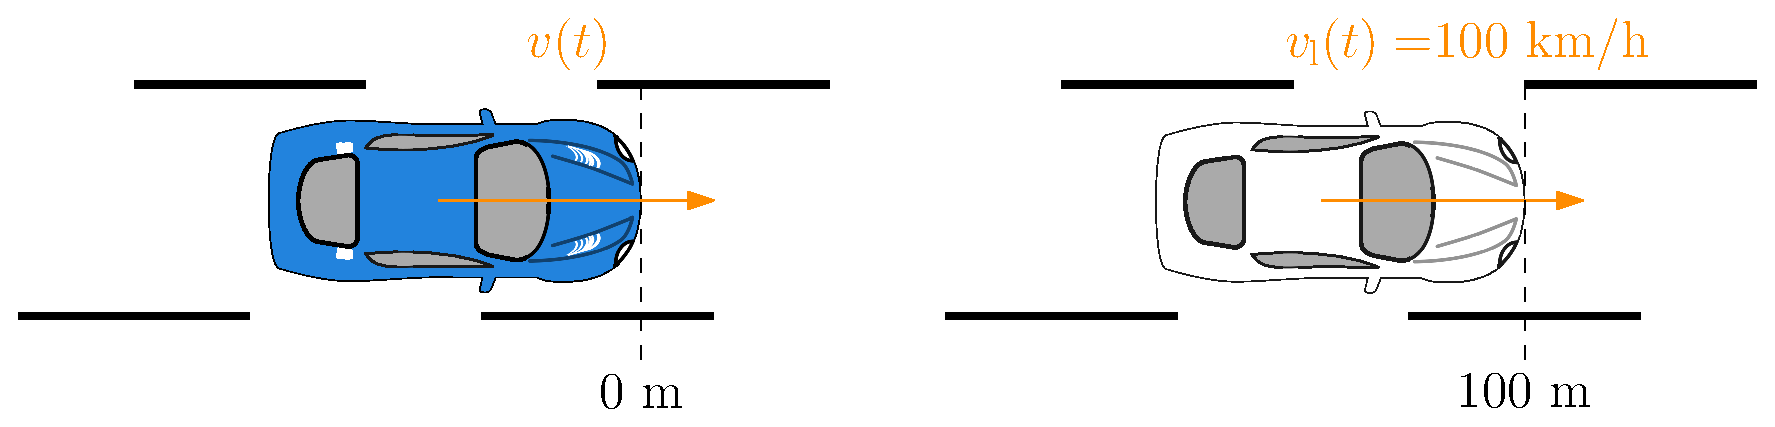
\includegraphics[width=.95\textwidth]{common/basic_2_car}
		\caption{Basic setup with 2 cars}
		\label{fig:basic2car}
	\end{figure}
	The leading car has a constant 100 km/h velocity. The following car - which is modeled with IDM - has an initial velocity of 100 km/h as well. The second car is 100 meters behind the other car. The parameters of following car can be seen in Table \ref{tab:idm_params}. The parameters have been chosen based on literature from [TODO:reference here].
	\begin{table}[ht]
		\begin{center}
			\begin{tabular}{ |c|c|c| }
				\hline
				$a_{\rm max}$ & $1.5$ & $\rm m/s^2$ \\
				$b_{\rm max}$ & $1.67$ & $\rm m/s^2$ \\
				$v_{\rm d}$ & $130$ & km/h \\
				$T$ & $1.8$ & s \\
				$h_0$ & $2$ & m \\
				$\rm \delta$ & $4$ & - \\
				$L$ & $4.5$ & m \\
				\hline
			\end{tabular}
		\end{center}
		\caption{Intelligent Driver Model parameters}
		\label{tab:idm_params}
	\end{table}
	The simulation was run until 100 seconds. Figure \ref{fig:basic2car_case_1} shows the result. The initial gap between the cars is greater than the second car's desired headway, consequently it will accelerate. The gap between the vehicles starts to decrease. At a certain time (around $t =$ 10) the second car starts to decelerate slowly based on the velocity difference and the decreasing headway. It will reach the desired safe gap at some point and will have exactly the same speed as the car before. It will maintain its desired headway.
	\begin{figure}
		\centering
		\begin{minipage}{.5\textwidth}
			\centering
			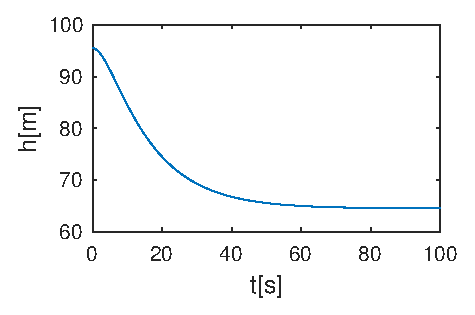
\includegraphics{ee/basic_2_car_headaway_case_1_2}
		\end{minipage}\hfill
		\begin{minipage}{.5\textwidth}
			\centering
			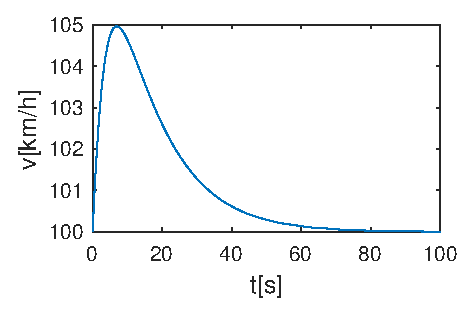
\includegraphics{ee/basic_2_car_velocity_case_1_2}
		\end{minipage}
		\caption{Following car's headway and velocity in Setup 1}
		\label{fig:basic2car_case_1}
	\end{figure}

	Another simulation was run with the same configuration except the initial headway was changed to 40 meters. Figure \ref{fig:basic2car_case_2} shows the result.
	\begin{figure}
		\centering
		\begin{minipage}{.5\textwidth}
			\centering
			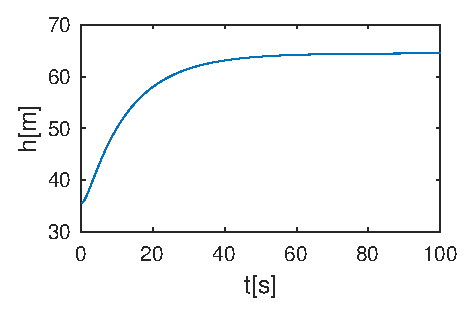
\includegraphics{ee/basic_2_car_headaway_case_2_2}
		\end{minipage}\hfill
		\begin{minipage}{.5\textwidth}
			\centering
			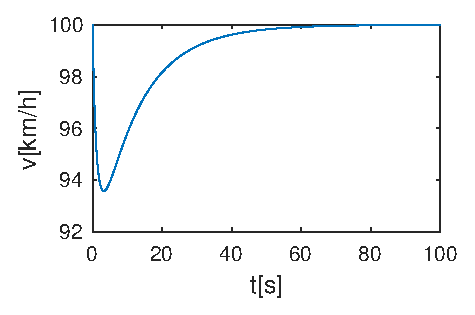
\includegraphics{ee/basic_2_car_velocity_case_2_2}
		\end{minipage}
		\caption{Following car's headway and velocity in Setup 2}
		\label{fig:basic2car_case_2}
	\end{figure}
